\documentclass[sigconf]{acmart}
%%% Local Variables:
%%% ispell-local-dictionary: "english"
%%% End:

\usepackage{booktabs} % For formal tables
\usepackage{graphicx}
\usepackage{rotating}

\begin{document}
\title{A modern, event-based architecture for distributed evolutionary algorithms}

\author{Juan-Juli\'an Merelo-Guerv\'os}
\orcid{1234-5678-9012}
\affiliation{%
  \institution{Universidad de Granada}
  \streetaddress{Daniel Saucedo Aranda, s/n}
  \city{Granada}
  \country{Spain}
}
\email{jmerelo@ugr.es}

\author{Jos\'e-Mario Garc\'ia-Valdez}
\affiliation{%
  \institution{Instituto Tecnol\'ogico de Tijuana}
  \streetaddress{Calzada Tecnol\'ogico, s/n}
  \city{Tijuana}
  \country{Mexico}
}
\email{mario@tectijuana.edu.mx}

% The default list of authors is too long for headers.
\renewcommand{\shortauthors}{JJ Merelo et al.}


\begin{abstract}
In this paper we introduce KafkEO, a cloud native evolutionary algorithms
framework that is prepared to work with population-based metaheuristics by using
micro-populations and stateless services as the main building
blocks; KafkEO is an attempt to map the traditional evolutionary
algorithm to this new cloud-native format.
\end{abstract}

\begin{CCSXML}
<ccs2012>
<concept>
<concept_id>10003752.10003809.10003716.10011136.10011797.10011799</concept_id>
<concept_desc>Theory of computation~Evolutionary algorithms</concept_desc>
<concept_significance>500</concept_significance>
</concept>

<concept>
<concept_id>10010520.10010521.10010537.10003100</concept_id>
<concept_desc>Computer systems organization~Cloud computing</concept_desc>
<concept_significance>500</concept_significance>
</concept>
\end{CCSXML}

\ccsdesc[500]{Theory of computation~Evolutionary algorithms}

\ccsdesc[500]{Computer systems organization~Cloud computing}

\ccsdesc[300]{Computing methodologies~Distributed algorithms}

\keywords{Cloud computing, microservices, distributed computing,
  event-based systems, stateless algorithms, functions as a service.}


\copyrightyear{2018}
\acmYear{2018}
\setcopyright{rightsretained}
\acmConference[GECCO '18 Companion]{Genetic and Evolutionary Computation Conference Companion}{July 15--19, 2018}{Kyoto, Japan}
\acmBooktitle{GECCO '18 Companion: Genetic and Evolutionary Computation Conference Companion, July 15--19, 2018, Kyoto, Japan}\acmDOI{10.1145/3205651.3205719}
\acmISBN{978-1-4503-5764-7/18/07}

\maketitle

\section{Introduction}

In general, Cloud based frameworks have tried to achieve functional equivalence with parallel or sequential versions of EAs \cite{salza2017ccube,de2017parallel,10.1007/978-3-319-32149-3_46,de2015scalable}. Besides these implementations using well known cloud services, there are new computation models for evolutionary algorithms
that are not functionally equivalent to a canonical EA, but have
proved to work well in these new environments. Pool based EAs,
\cite{bollini1999distributed}, have been used for new
frameworks such as EvoSpace \cite{García-Valdez2015}, and proved to be
able to accommodate all kinds of ephemeral and heterogeneous
resources. In the serverless, event based types of architectures we are going to
be targeting in this paper, there has been so far no work that we know
of. Similar setups including microservices have been employed by Salza et
al. \cite{salza2017ccube}; however, the serverless system adds a layer
of abstraction to event-based queuing systems such as the one employed
by Salza by reducing it to functions, messages and rules or
triggers.

In this paper we want to introduce KafkEO, a serverless framework for
evolutionary algorithms and other population-based systems. The main
design objective is to leverage the scaling capabilities of a
serverless framework, as well as create a system that can be deployed
on different platforms by using free software. Our intention has
also been to create an algorithm that is functionally equivalent to an asynchronous parallel, island-based, EA, which can use parallelism and at the same time reproduce mechanisms that are akin to migration. The island-based
paradigm is relatively standard in distributed EA applications, but in our case,
we have been using it since it allows for better parallelism
and thus performance, at the same time it makes keeping diversity
easier while needing less free parameters to tune.
The rest of the paper is organized as follows. Next we present The KafkEO Event based framework and in section \ref{sec:con} conclusions
and future lines of work.


\section{The KafkEO Event based framework}
\label{sec:methods}
%
\begin{figure*}[h!tbp]
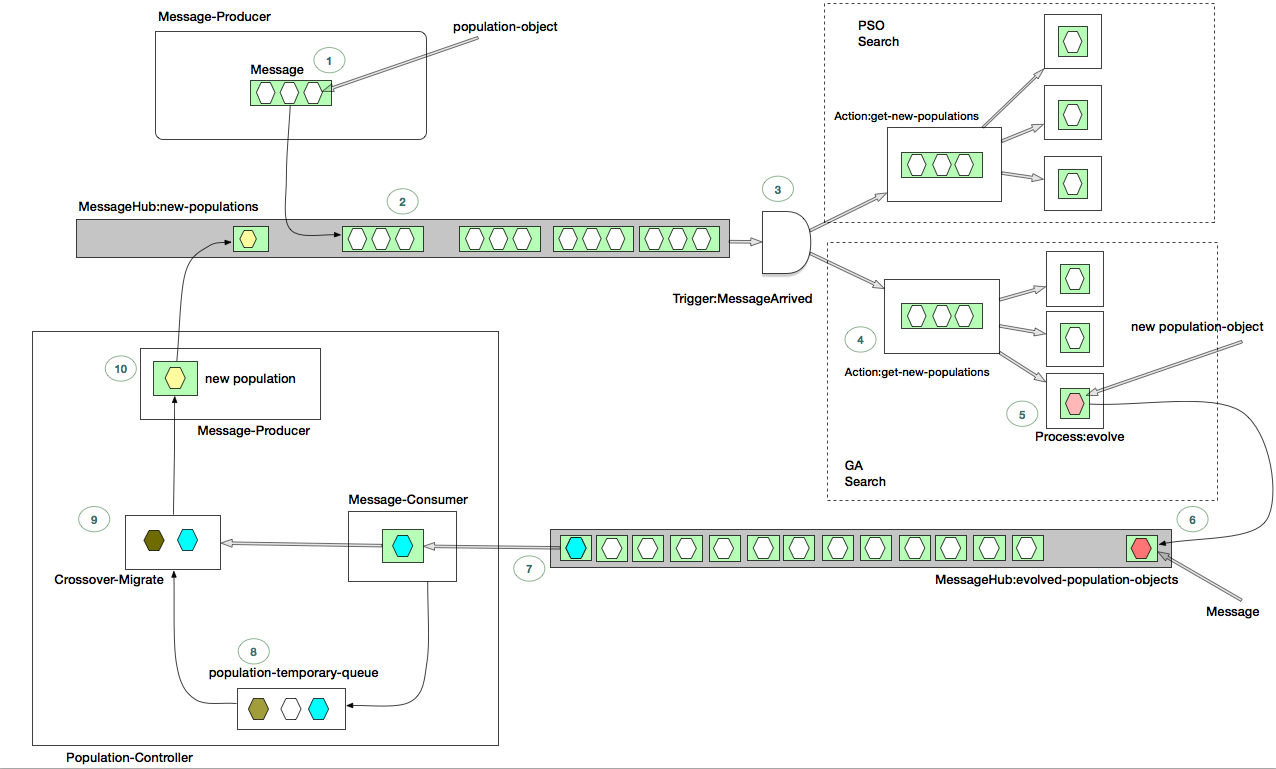
\includegraphics[width=0.75\textwidth]{img/kafkEO.png}
\caption{A flow diagram of KafkEO, showing message routes, MessageHub
  topics and the functions that are being used.}
\label{fig:kafkeo2}
\end{figure*}
%

The evolutionary algorithm mapped over this architecture is
represented in Figure \ref{fig:kafkeo2}. The main
design challenge is to try and map an evolutionary algorithm to a
serverless, and then stateless, architecture. That part is done in
points 1 through 5 of Figure \ref{fig:kafkeo2}. The beginning of the
evolution is triggered from outside the serverless framework (1) by
creating a series of Population objects, which we pack (2) to a message in the
{\sf new-populations} {\em topic}. The arrival of a new population
package sets off the {\sf MessageArrived} trigger (3), that is bound to
the actions that effectively perform evolution. In this case we
feature GA and PSO algorithms, although only GA has been implemented
for this paper. Any number of actions can be triggered in parallel by the same message,
and new actions can be triggered while others are still working; this phase is
then self-scaling and parallel by design.

Population objects are extracted from the message and, for each, a call to
an {\em evolve} process is executed in parallel. The {\em evolve} process
consists of two sequential {\em actions} (5), first, the {\em GA Service} function that
runs a GA for a certain number of generations, producing a new evolved
object, which is then sent to the second action called {\em Message Produce}
 responsible of sending the object to the {\sf evolved-population-objects}
 message queue.  The new Population object (6) includes
 the evolved population and also metadata such as a flag indicating
whether the solution has been found, the best individual, and information
about each generation. With this metadata a posterior analysis of the experiment
can be achieved or simply generating the files used by the BBOB Post-processing scripts.

This queue is polled by a service outside the serverless framework, called
{\sf Population-Controller}. This service needs to be stateful, since
it needs to wait until several populations are ready to then mix them (in
step \#9 in Figure \ref{fig:kafkeo2}) to produce a new population, that is the result of selection
and crossover between several populations coming from the {\sf
  evolved-population-objects} message queue. Eventually, these mixed
populations are returned to the initial queue to return to the {\em
  serverless} part of the application. Another task of the
  {\sf Population-Controller} is to start and stop the experiment. The service must
  keep the number of Population objects received, then after
  a certain number is reached, the controller stops sending new messages to the
  {\sf new-populations} {\em topic}. It is important to note, that because of
  the asynchronous nature of the system, several messages could still
  arrived after the current experiment is over. The controller must only
  accept messages belonging to the current process.

% consists essentially on a single function, a single topic
% in the MessageHub and a single kind of message, which includes a whole
% population along with metadata. The function performs a series of
% generations on the population, using a canonical algorithm with
% mutation and crossover. If it finds the solution, in our case, the
% minimum fitness, it sets a flag indicating it has found it so that it
% propagates to different instances of the population; in any case, it
% sends the whole evolved population as a message to the MessageHub, to
% be propagated to the other instantiations on the function.

This would be functionally equivalent to a sequential algorithm except
for the fact that, between two calls to the {\sf get-new-populations}
function, several
population-messages have been received in the message queue. In fact,
every call the {\sf Crossover-migrate} function receives several populations, which
have to be merged to generate several new populations. This {\em merging} step
before starting evolution takes the place of the {\em migration} phase
and allows this type of framework to work in parallel, since several
instances of the function might be working at the exact same time; the
results of these instances are then received back by every one of the
instances.



\section{Conclusions}
\label{sec:con}

This paper is intended to introduce a simple proof of concept of a
serverless implementation of an evolutionary algorithm. The main
problem with this algorithm, shared by many others, is to turn an algorithm that has state (in the form of loop variables or anything
else) into a stateless system. In this initial proof of concept we have
opted to create a stateful {\em mixer} outside the serverless (and
thus stateless) platform to be able to perform {\em
  migration} and mixing among populations. A straightforward first step
would be to parallelize this service so that it can respond faster to
incoming evolved populations; however, this scaling up should be done
by hand and a second step will be to make the architecture totally
serverless by using functions that perform this mixing in a stateless
way. This might have the secondary effect of simplifying the messaging
services to a single topic, and making deployment much easier by
avoiding the desktop or server back-end we are using now for that
purpose.


\begin{acks}
This paper has been supported in part by
\href{http://geneura.wordpress.com}{GeNeura Team}, 
projects TIN2014-56494-C4-3-P (Spanish Ministry of Economy and
Competitiveness) and DeepBio (TIN2017-85727-C4-2-P).
\end{acks}


\bibliographystyle{ACM-Reference-Format}
\bibliography{serverless}

\end{document}
